\documentclass[amsmath,amssymb,10pt,twocolumn,eqsecnum]{revtex4}
\usepackage{ graphicx, amsmath, amsmath, amssymb, subfigure}
\input{defs}
\newcommand{\comment}[1]{{\color{red}[#1]}}
\newcommand{\note}[1]{{\color{blue}#1}}
\newcommand{\todo}[1]{{\color{blue}#1}}
\newcommand{\Mpsq}[0]{{\qsubrm{M}{pl}^2}}
\usepackage[breaklinks, colorlinks, citecolor=blue]{hyperref}
\linespread{1}
\begin{document}

 

\title{Predicting Armageddon for the sequestered Universe}
\author{Jonathan A. Pearson}
\email{j.pearson@nottingham.ac.uk}
\affiliation{School of Physics \& Astronomy, University of Nottingham, Nottingham, NG7 2RD, U.K.}

\date{\today}


\begin{abstract} 
In conversation with Adam Moss, Tony Padilla, Nemanja Kaloper, Jolyon Bloomfield.

\end{abstract}

\maketitle
%\tableofcontents
\section{Introduction}
The recently proposed \textit{vacuum sequestering} solution to the cosmological constant problem \cite{Kaloper:2013zca, Kaloper:2014dqa, Kaloper:2014fca} needs confronting to data in order to have its free parameters constrained. A consequence of this is that we will obtain predictions for the date of  Universal Armageddon, as well as a prediction for the maximum size of the Universe.

Some observational properties of sequestering solutions have been studied in \cite{Avelino:2014nqa, Avelino:2014aea, Kluson:2014tma}.

%\subsection{Review of the model}
We will use a linear quintessence potential, $V(\phi) =  {m}^3\phi$ to provide the dark energy dynamics which will cause the Universe to collapse. In some sense, this enables sequestering solutions to be found in the theory. This model was studied \cite{Kallosh:2003bq} independantly of requiring sequestering solutions.

The equations of motion in spatially flat FRW space-time  are
\bse
\label{frw-eqnsofmotion}
\bea
3\Mpsq H^2 =  {\rho}{ } + \half \dot{\phi}^2 +m^3\phi,
\eea
\bea
3\Mpsq \dot{H} = - \frac{3}{2}\left(  {\rho}{ } +  {p}{ } + \dot{\phi}^2\right),
\eea
\bea
\ddot{\phi} + 3 H \dot{\phi} +m^3=0,
\eea
\ese
\comment{add in spatial curvature}
in which overdots denote derivatives with respect to coordinate time, $H \defn \dot{a}/a$ defines the Hubble parameter, and $(\rho, p)$ are the energy density and pressure of matter sources (including baryons, CDM, and radiation).

Field configurations which are \textit{sequestering solutions} are the solutions to (\ref{frw-eqnsofmotion}) for whom the constraint
\bea
\label{eq:seq_constraint}
\langle\dot{\phi}^2\rangle - 4m^3 \expec{\phi} + \expec{3 {p}{ } -  {\rho}{ }} = 0,
\eea
is satisfied. In (\ref{eq:seq_constraint}), the symbol $\expec{Q}$ is defined as the historic integral; in the FRW background the historic integral is
\bea
\expec{Q} \defn \frac{\int_{\qsubrm{t}{bang}}^{\qsubrm{t}{crunch}} \dd t \,a(t)^3\, Q(t)}{\int_{\qsubrm{t}{bang}}^{\qsubrm{t}{crunch}} \dd t\, a(t)^3}.
\eea
Note that the start-point of the integrals is the ``big bang'', and the end-point is the ``big-crunch''. The dark energy theory considered here is such that the Universe is guaranteed to end in a crunch. The constraint (\ref{eq:seq_constraint}) is equivalent to  the vanishing of the historic integral of the Ricci scalar
\bea
\label{eq:vanish_R}
\expec{R} = 0
\eea
on sequestering solutions.




 
 

{\renewcommand{\arraystretch}{1.4}
\begin{table}%[b] 
%\begin{andptabular}{X[4c]X[4c] }%
\begin{center}
\begin{tabular}{||c |  c ||}
%{Summary  of    commonly used symbols}
\hline
\textbf{Parameter} & \textbf{Fiducial value} \\
\hline
Hubble, $h$ ($H_0 = 100h$km/s/Mpc) & 0.7 \\\hline
Current matter fraction, $\qsubrm{\Omega}{m}h^2$ &0.137  \\\hline
Current baryon fraction, $\qsubrm{\Omega}{b}h^2$ &0.02240  \\\hline
Current curvature fraction, $\qsubrm{\Omega}{k}h^2$ &0.0 \\\hline
Effective rel.dofs, $\qsubrm{N}{eff}$ &3.046 \\\hline
Photon temperature, $T_{\gamma}$ & 2.72548 \\\hline\hline
Scalar field initial conditions, $(\phi_0, \dot{\phi}_0)$ &(1.5, 0.01) \\\hline
\end{tabular}\caption{Fiducial values of the parameters.}\label{tab:fid_params}
\end{center}
\end{table}
}

 
\section{Updated observational constraints on the GR $V = m^3\phi$ theory}
Here we present updated constraints on the  $V = m^3\phi$ quintessence theory in pure GR; i.e., the equations of motion are given by (\ref{frw-eqnsofmotion}) and we simply aren't bothered about the sequestering constraint.

In \fref{fig:plots-like}(a) we plot the likelihood on the $(m^3, \qsubrm{\Omega}{k}h^2)$-plane. We observe that there is some region in this space which is observationally preferred. 

\begin{figure*}[!t]
      \begin{center}
{\includegraphics[scale=0.5]{images/test22_2_L_GR}}
      \end{center}
\caption{Using  SN1a+BAO+WMAP data   to pick out observationally preferred        Universes with with a quintessence dark energy component with linear potential. We emphasise that these are not MCMC likelihoods, and all other cosmological and model parameters have been held fixed to their fiducial values. We plot the observationally preferred values of $(m^3, \qsubrm{\Omega}{k}h^2)$ without imposing the sequestering constraint. This shows that smaller values of $m^3$ require larger (more negative) spatial curvatures for observationaly compatibility.   }\label{fig:plots-like}
\end{figure*}

\comment{Get MCMC code to spit out $\qsubrm{a}{max}$ \& $\qsubrm{t}{max}$}

\section{Observational constraints on the sequestering theory} 
In this section we describe properties of universes which have sequestering solutions. We then move on to confront the model with   data to observationally constrain the freedom in the sequestering model. This ultimately leads to being able to set a date for Armageddon.

\subsection{Numerical implementation}

We solve the equations of motion (\ref{frw-eqnsofmotion}) using the  {\tt deevolve} code developed with J. Bloomfield; the equations are evolved in conformal time until the Universe collapses at $a=0$.  The material content is: matter, radiation, and quintessence scalar field with linear potential. This provides a number of parameters which  parameterize the solutions: 
\bea
\rbm{p} = \left\{ \qsubrm{\Omega}{m}, \,\qsubrm{\Omega}{r},\,m,\,\phi_0, \,\dot{\phi}_0 \right\}.
\eea
We include the initial values of the scalar field, $\phi_0$, and its time derivative, $\dot{\phi}_0$ in the list of free parameters; the quintessence model does not nessecarily have attractor solutions, and so varying the initial conditions should be expected to vary the final outcome. The fiducial values of these parameters are given in \tref{tab:fid_params}. Using a simple algorithm we explain below, we search the parameter space for the combination of model and cosmological parameters for whose solutions the sequestering constraint (\ref{eq:vanish_R}) holds. 

 \begin{figure*}[!t]
      \begin{center}
	\subfigure[\, $\log_{10}|\langle R\rangle|$]{\includegraphics[scale=0.5]{images/wl/test22_2_HIR}} \qquad
      	\subfigure[\, $10^2(1+w_0)$]{\includegraphics[scale=0.5]{images/wl/test22_2_w0}}
	\subfigure[\, Maximum size of the Universe, $\qsubrm{a}{max} $]{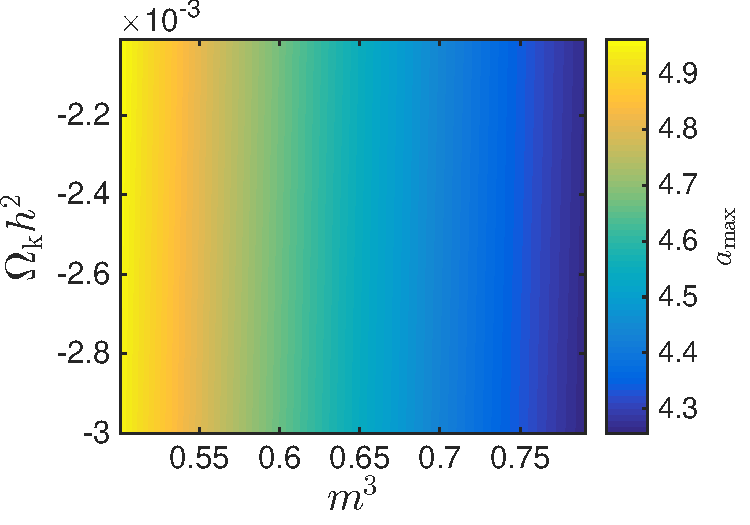
\includegraphics[scale=0.5]{images/wl/test22_2_amax}}\qquad
	\subfigure[\, Age of the Universe at collapse, $\qsubrm{t}{max} $]{\includegraphics[scale=0.5]{images/wl/test22_2_tmax}}
      \end{center}
\caption{Obtaining the  properties of a sequestering Universe.  In (a) we  show the region of $(m^3,\qsubrm{\Omega}{k}h^2)$-space which are compatible with a sequestering solution. This is done by computing the value of $\langle R\rangle$: the regions where this quantity is small contain the sequestering solutions, and is denoted with the dotted line. One should note that $\langle R\rangle$ changes sign either side of the dotted line. In (b) we show the value of the current value of the dark energy equation of state, $w_0$.  From (c) and (d) we see that a given location in the $(m^3,\qsubrm{\Omega}{k}h^2)$-plane can be interpreted as a maximum size of the Universe,   $\qsubrm{a}{max}$, and age of the Universe at Armageddon, $\qsubrm{t}{max}$.}\label{fig:plots3}
\end{figure*}

 
 
%
%For reference,  the historic average in conformal time is
%\bea
%\expec{Q} \defn \frac{\int_{\qsubrm{\tau}{bang}}^{\qsubrm{\tau}{crunch}} \dd \tau \,a(\tau)^4\, Q(\tau)}{\int_{\qsubrm{\tau}{bang}}^{\qsubrm{\tau}{crunch}} \dd \tau\, a(\tau)^4}.
%\eea
%The crunch-time $\qsubrm{\tau}{crunch}$ is defined to be where $a\left(\qsubrm{\tau}{crunch}\right)=0$.

Numerical solutions are not entirely simple to obtain, mainly for the reason that we require solutions which are valid from the big bang to the crunch. These end-points are singular points in the equations of motion, as well as all known and assumed physics being expected to break down: no-one expects the FRW geometrical ansatz to hold true infinitesimally close to the end of the Universe. And so, in practice we evolve as close to these singular end-points as is numerically viable, and check that any resulting conclusions are independant (or at least converge) of the cut-offs imposed.
 
We first provide properties of not-nessecarily-sequestering solutions, and show how one can detect a sequestering solution. For a first illustrative example, we fix all parameters, except $m^3$ and the spatial curvature, $\qsubrm{\Omega}{k}h^2$. The equations of motion are solved for each combination of the pairs of parameters. This allows us to compute diagnostic quantities such as the values of $\langle R\rangle$, current value of the dark energy equation of state parameter $w_0$, maximum size of the Universe, and the age of the Universe at Armageddon.

These diagnostic quantities are presented in \fref{fig:plots3}. In (a) we show how the historic integral $\langle R\rangle$ depends upon the two parameters we have dialled. We find that $\langle R\rangle=0$ is obtained within the window of parameter space we have shown: the zero lies along (or very close to) the dashed-line we have superimposed over the plot. The combination of parameters which lies along this dashed line  are the sequestering solutions. Although this plot shows the log of the magnitude of $\langle R\rangle$, plotting the sign of $\langle R\rangle$ reveals identical behavior. Simple empirical analysis of this plot reveals that sequestering solutions lie on the line given by
\bea
\qsubrm{\Omega}{k}h^2 = -10^3\left( 1.1\, m^3 + 1.8\right).
\eea
This also shows that sequestering solutions require spatial curvature. Numerically, it is rather difficult to exactly hone in on the region of parameter space which has an exact (or is arbitrarily close to a) zero. This issue is entirely numerical in nature, and can be elucidated by inspecting (c) since see that  these universes are never particularly big: this has the effect of enhancing the problematic influence of the singularity at the crunch. However, we can remain confident that sequesting solutions live within the band shown. 

By studying (b) we also see that these models all have $w_0$ rather close to $w_0 \sim -1$. It should be clear that reducing $m^3$ has the effect of making the Universe larger and older before Armageddon. It will also push $w_0$ closer to $-1$. Notice that the sequestering solutions induce a correlation between spatial curvature and $m^3$, and therefore between the spatial curvature and $w_0$.

One   may ask why we looked at this window in parameter space, rather than a window for whom the universes are much larger, which ameliorates the numerical problems associated with the crunch. The answer is that we focussed on the region which is observationally compatible.   
 
\subsection{Sequestering solutions}
The analysis of the previous section gives motivation for our algorithm to find sequestering solutions. We numerically \textit{derive} the value of spatial curvature required to yield a sequestering solution: we pick a desired set of cosmological and model parameters, and tune the value of $\qsubrm{\Omega}{k}h^2$ until the equations have solutions which are  ``sequestering'' to a desired level of accuracy. In \fref{likelihood_sequestering_sweep} we present results of an analysis with this philosophy.

In \fref{likelihood_sequestering_sweep}(b) we provide the value of spatial curvature which is derived to give a sequestering solution, as a function of $m^3$ (all other parameters are fixed to their fiducial values). In \fref{likelihood_sequestering_sweep}(a) we present the observationally derived likelihoods for a range of values of $m^3$ for the sequestering solutions: it is clear that a particular value of the mass is picked out. The maximum size of these universes, as well as the age of the universe at Armageddon, can be computed, and are given in \fref{likelihood_sequestering_sweep}(c) and (d) respectively. On those plots we have also highlighted the regions which have maximum likelihood (largest likelihoods are marked on with red, lower with blue, and lowest with green). Again, it is clear that the data picks out a preffered maximum size of the universe, and date for Armageddon.

\subsection{Observational constraints}
\comment{DO MCMC ANALYSIS}
 \begin{figure*}[!t]
      \begin{center}
      	\subfigure[\, Likelihood ]{\includegraphics[scale=0.4]{images/seqs_1d/test22_33_L}} \qquad
	\subfigure[\, Derived spatial curvature ]{\includegraphics[scale=0.4]{images/seqs_1d/test22_33_Omk}}\\
	\subfigure[\, $\qsubrm{a}{max}$ ]{\includegraphics[scale=0.4]{images/seqs_1d/test22_33_amax}} \qquad
	\subfigure[\, $\qsubrm{t}{max}$ ]{\includegraphics[scale=0.4]{images/seqs_1d/test22_33_tmax}} 
      \end{center}
\caption{Using data to predict properties of sequestered universes. Here we dial the spatial curvature until a sequestered solution is found for a given set of initial data. In (a) we plot the likelihood from SN1a+BAO+WMAP data, and in (b) the spatial curvature required to yield sequestering solutions. In (c) we plot the maximum size of the Universe, and the colours denote the observational likelihood on the sequestering solutions (blue is $L > 0.6$ and red $L > 0.9$). Similarly, (d) is the age of the Universe at Armageddon, on sequestering solutions. }\label{likelihood_sequestering_sweep}
\end{figure*}

\section{Discussion} 

\bibliographystyle{JHEP}
\bibliography{refs}

\end{document}